%In the previous section each component of the system was modeled with differential and algebraic equations. The modeling format is such that every component takes some inputs, and from those calculates some states and some outputs which are used for the adjacent components. In order to make a complete non-linear model it is necessary to connect the inputs and outputs of the system. This section provides insight into how components are interfaced and collected into a complete non-linear state space form.

In the previous section each component of the system was modeled with differential and algebraic equations. The equations for each component generally require inputs from adjacent components, to generate outputs used in adjacent components. The aim of this section is to create a state space model which encapsulates all these interconnections. The model is expected to be non-linear as a direct result of the generally non-linear physics that describe thermodynamic systems. \cref{sec:mod_lin} will cover how the model is linearised.\\

The block diagram in \cref{fig:Block_diagram_inout} gives an overview of the system interface variables and states. In the diagram the component interface variables are split out to show which variables are used as inputs and outputs for each component. Some inputs to components are highlighted in red to signify that they are not found as outputs from a component. Steady State values (operating points) are used for these. The values are taken from the the high-fidelity simulation in steady state. Blue variables are outputs of components that are not used by the adjacent component. Each component block also contains the names of the states they contain.

\begin{figure}[h!]
	\centering
	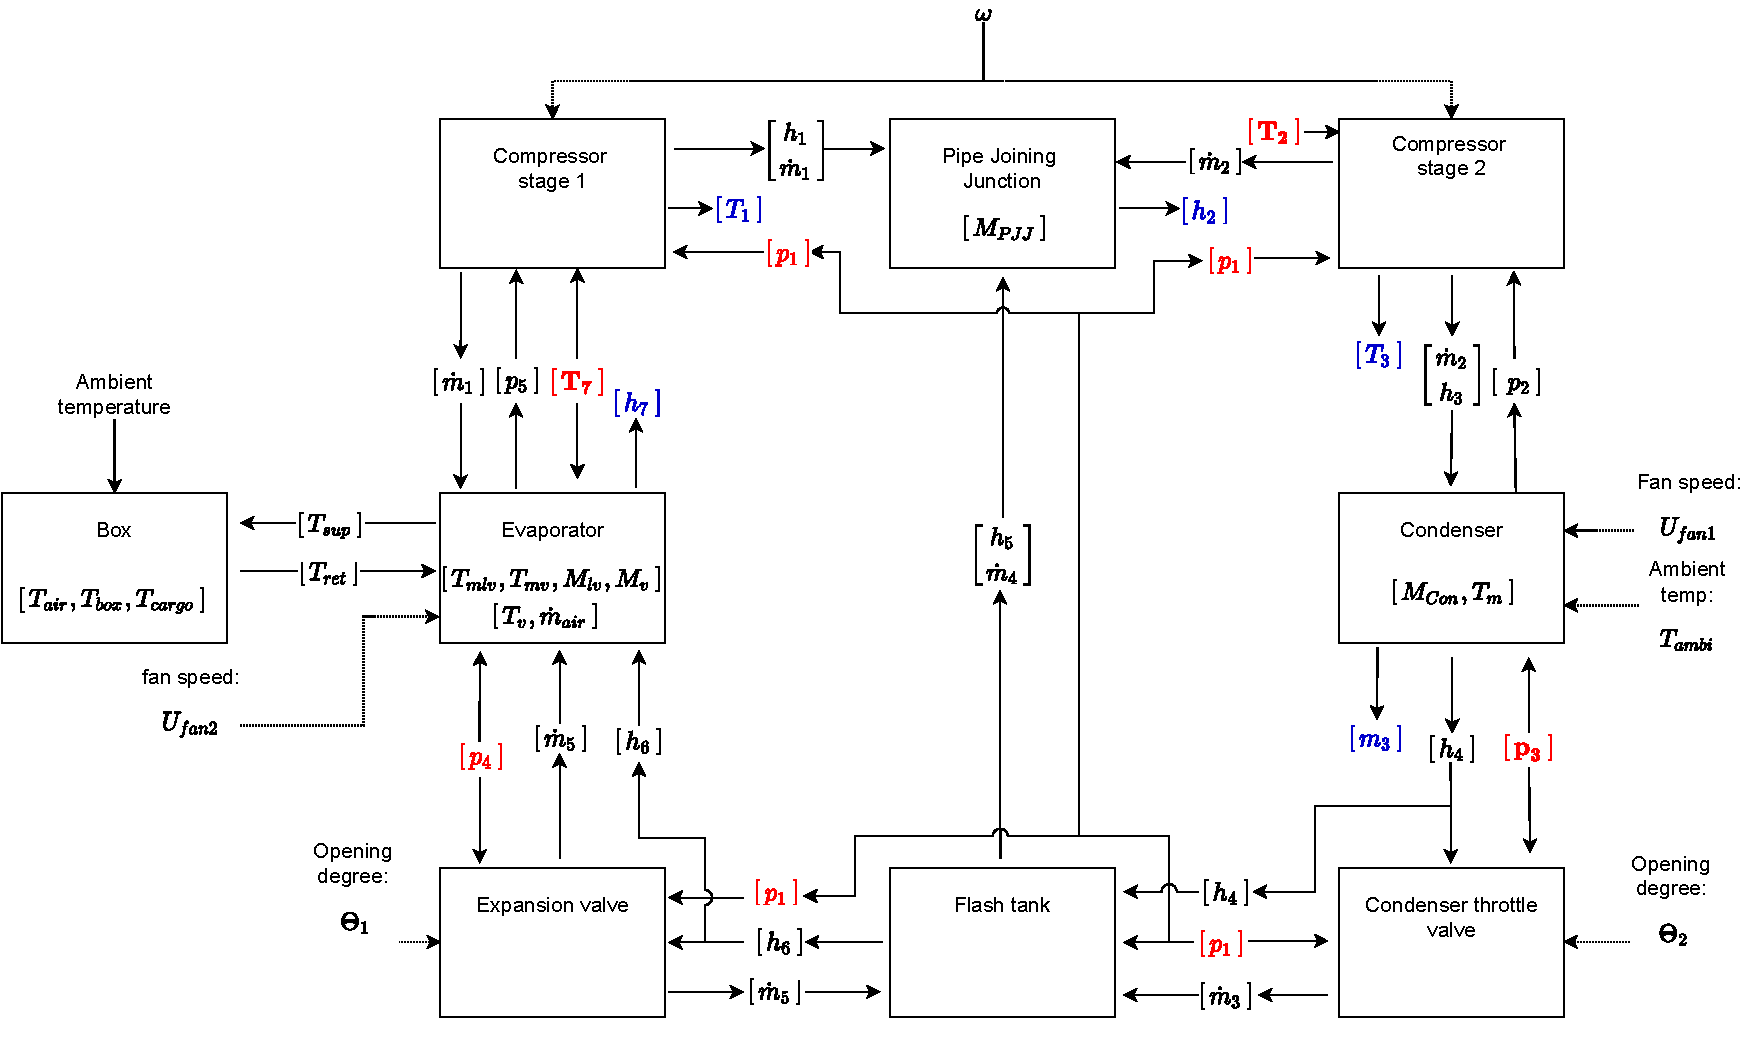
\includegraphics[width=1\textwidth]{Graphics/Block_Diagram_inout_flowValveVersion.pdf}
	\caption{Block diagram of input/output relationship of interface variables}
	\label{fig:Block_diagram_inout}
\end{figure}

\todo{write about what problems lie ahead. Conclude on the connections in the diagram and the steady state values and operating points. Can not be generalised to other operating points..}

\newpage

\subsubsection{Mathematical formulation of non-linear state space model} \label{sec:non_lin_model}
As described in \cref{sec:mod}, there are large variances in dynamical speed across the system. Therefore, the fast components were defined algebraically, while the slow dynamics were modeled with a mix of differential equations and algebraic equations. The fast components are considered the compressors and the valves.

The variables are differentiated in the differential equations in \cref{sec:mod_comp_mod}, are the system states. These are combined as a state vector $x$. The controlled inputs are likewise combined in the input vector $u$. These vectors are seen in \cref{eq:xu}.
%\begin{equation} \label{eq:xu} \renewcommand{\arraystretch}{2.4}
%	x = \begin{bmatrix}
%		M_{pjj}			\\				%pjj
%		M_{con} 		\\				%condenser
%		T_m 			\\				%condenser
%		\dot{m}_{air}	\\				%evaporator
%		T_{mlv}			\\				%evaporator
%		T_{mv}			\\				%evaporator
%		M_{lv}			\\				%evaporator
%		M_v				\\				%evaporator
%		T_{air}			\\				%box
%		T_{box}			\\				%box
%		T_{cargo}		\\				%box
%	\end{bmatrix} \;\;\;\;\;\;\;\;\;
%	u = \begin{bmatrix}
%		\Theta_1			\\				%pjj
%		\Theta_2 		\\				%condenser
%		U_{fan_1}			\\				%condenser
%		U_{fan_2}	\\				%evaporator
%		\omega			\\				%evaporator
%\end{bmatrix}
%\end{equation}
\begin{equation}  \label{eq:xu}
	\begin{split}
		x &= \begin{bmatrix}
			M_{pjj}				&		%pjj
			M_{con} 			&		%condenser
			T_m 				&		%condenser
			\dot{m}_{air}		&		%evaporator
			T_{mlv}				&		%evaporator
			T_{mv}				&		%evaporator
			M_{lv}				&		%evaporator
			M_v					&		%evaporator
			T_{air}				&		%box
			T_{box}				&		%box
			T_{cargo}					%box
		\end{bmatrix}^T \\
		u &= \begin{bmatrix}
			\Theta_1			&			%pjj
			\Theta_2 			&			%condenser
			U_{fan_1}			&			%condenser
			U_{fan_2}			&			%evaporator
			\omega							%evaporator
		\end{bmatrix}^T
	\end{split}
\end{equation}


We define a function $f(x,u)$ as a vector of the state derivatives:
% F: States
% ------------------------------------

\begin{equation} \label{eq:f_noSub} \renewcommand{\arraystretch}{2.4}
	f(x,u) =  \dfrac{d}{dt} \begin{bmatrix}
		M_{pjj}			\\				%pjj
		M_{con} 		\\				%condenser
		T_m 			\\				%condenser
		\dot{m}_{air}	\\				%evaporator
		T_{mlv}			\\				%evaporator
		T_{mv}			\\				%evaporator
		M_{lv}			\\				%evaporator
		M_v				\\				%evaporator
		T_{air}			\\				%box
		T_{box}			\\				%box
		T_{cargo}		\\				%box
		T_v				\\				%evaporator

	\end{bmatrix}
	=
	\begin{bmatrix}
		\dot{m}_1(M_{v}, \omega) + \dot{m}_4(T_m,\Theta_1,\Theta_2,\omega) - \dot{m}_2(\omega) \\										%pjj
		\dot{m}_{2}(\omega) - \dot{m}_{3}(\Theta_2)	\\												%condenser
		\dfrac{Q_{rm}(T_m) - Q_{ma}(T_{ambi}, T_m, U_{fan1})}{M_m \cdot Cp_m} \\									%condenser
		\dfrac{\bar{\dot{m}}_{air}(U_{fan2})  - \dot{m}_{air}(\dot{m}_{air})} {10s}		\\					%evaporator
		\dfrac{Q_{amlv}(T_{mv},T_{mlv},\dot{m}_{air})-Q_{mlv}(M_{lv},T_{mlv}) + Q_{mvmlv}(T_{mv},T_{mlv})}{M_m \cdot Cp_m \cdot \sigma(M_{lv})}        \\	%evaporator
		\dfrac{Q_{amv}(T_{air},T_{mv},U_{fan2},\dot{m}_{air}) - Q_{mv}(M_{lv},T_{mv}) - Q_{mvmlv}(T_{mv},T_{mlv})}{M_m \cdot Cp_m \cdot (1- \sigma(M_{lv}))}	\\	%evaporator
		\dot{m}_{5}(\Theta_1) - \dot{m}_{dew}(M_{lv},T_{mlv})		\\											%evaporator
		\dot{m}_{dew}(M_{lv},T_{mlv}) - \dot{m}_1(M_{v}, \omega)	\\												%evaporator
		\dfrac{Q_{ca}(T_{air},T_{cargo}) + Q_{ba}(T_{air},T_{box}) + Q_{fan}(U_{fan2}) - Q_{cool}(T_{air},T_{mv},T_{mlv},U_{fan2},\dot{m}_{air})}{M_{air} \cdot Cp_{air}} \\					%box
		\dfrac{Q_{amb}(T_{ambi},T_{box}) -  Q_{ba}(T_{air},T_{box})}{M_{box} \cdot Cp_{box}} \\							%box
		\dfrac{-Q_{ca}(T_{air},T_{cargo})}{M_{cargo} \cdot Cp_{cargo}}									\\	%box
		\bar{T_v}(M_{lv},T_{mv},T_{mlv},T_v) - T_v 
	\end{bmatrix}
\end{equation}

\cref{eq:f_noSub} is the set of equations that constitutes the non-linear state space representation of the refrigeration system. All the functions on the right most side of the equation, can be substituted with the algebraic equations from the modelling section. This is too extensive to fit into a single page, so it is omitted. In stead the functions on the right most side indicates which states in $ x $ and inputs in $ u $ that affects them. Additionally it is indicated if the functions are affected by the disturbance $ T_{ambi} $. The model contains 12 states, 5 control inputs and 1 disturbance. The next step in the project is now to validate the found non linear state space model.

\newpage
\subsection{Model verification}\label{sec:model-verification}
In order to validate the model found in \cref{eq:f_noSub}, a simulation of steady state was desired. The aim of the simulation was to confirm whether the model states acts stable, especially for the states that affects the system outputs, $T_v$ and $T_{air}$.

When referring to \cref{fig:Block_diagram_inout}, it is apparent that in order to simulate the system, some steady state variables had to be introduced in order to be able to perform the simulation model. These are all the red variables in \cref{fig:Block_diagram_inout}. Additionally, the inputs needed to be set to steady state values.The concrete numeric values for both the inputs and the steady state variables where found in the HiFi simulation after 5000 s. Finally, the states needed to be initialised in a sensible manner, and these were estimated with common sense, and based on the pressures, temperatures and volumes of the control volumes. All of the necessary values for the simulation is found in the tables below. \\


\begin{tabular}{cc}
	\begin{minipage}{.3\linewidth}
		\centering
		\begin{tabular}{@{}lll@{}}
			\toprule
			\textbf{Variables} & \textbf{\begin{tabular}[c]{@{}l@{}}Numeric \\ values\end{tabular}} & \textbf{Unit} \\ \midrule
			$p_1$              & 0.44944                                                            & MPa           \\
			$p_3$              & 0.77637                                                            & MPa           \\
			$p_4$              & 0.19237                                                            & MPa           \\
			$T_2$              & 295.3925                                                           & K             \\
			$T_7$              & 267.6048                                                           & K             \\ \bottomrule
		\end{tabular}
	\end{minipage} &
	\begin{minipage}{.3\linewidth}
		\centering
		\begin{tabular}{@{}lcl@{}}
			\toprule
			\textbf{\begin{tabular}[c]{@{}l@{}}Initial \\ state values\end{tabular}} & \multicolumn{1}{l}{\textbf{\begin{tabular}[c]{@{}l@{}}Numeric \\ values\end{tabular}}} & \textbf{Unit} \\ \midrule
			$M_{pjj}$                                                                & 0.001                                                                                  & kg   \\
			$M_{con}$                                                                & 1                                                                                      & kg   \\
			$T_m$                                                                    & 302                                                                                    & K    \\
			$\dot{m}_{air}$                                                          & 0.25                                                                                   & kg/s \\
			$T_{mlv}$                                                                & 262                                                                                    & K    \\
			$T_{mv}$                                                                 & 273                                                                                    & K    \\
			$M_{lv}$                                                                 & 0.5                                                                                    & kg   \\
			$M_{v}$                                                                  & 0.0075                                                                                 & kg   \\
			$T_{air}$                                                                & 268.9                                                                                  & K    \\
			$T_{box}$                                                                & 278.15                                                                                 & K    \\
			$T_{cargo}$                                                              & 263.15                                                                                 & K    \\
			$T_{v}$                                                                  & 267.6048                                                                               & K    \\ \bottomrule
		\end{tabular}
	\end{minipage}
	\begin{minipage}{.3\linewidth}
		\centering
		\begin{tabular}{@{}lll@{}}
			\toprule
			\textbf{Inputs} & \textbf{\begin{tabular}[c]{@{}l@{}}Numeric \\ values\end{tabular}} & \textbf{Unit} \\ \midrule
			$\omega$        & 28                                                                 & \%            \\
			$\Theta_1$      & 19.4                                                               & \%            \\
			$\Theta_2$      & 12.1                                                               & \%            \\
			$U_{fan1}$      & 62.8                                                               & \%            \\
			$U_{fan2}$      & 63.8                                                               & \%            \\
			$T_{ambi}$        & 293.15                                                             & K             \\ \bottomrule
		\end{tabular}
	\end{minipage}
\end{tabular}\\


In the inspection of the time evolvement of the states in the simulation, the states will be paired in groups that make them relatable. We first illustrate some results that indicate that our model is flawed. As can be seen in \cref{fig:non_lin_sim_faulty_Mass} the refrigerant masses $M_{pjj}$ and $M_{con}$ are integrating over time.

\begin{figure}[h]
	\centering
	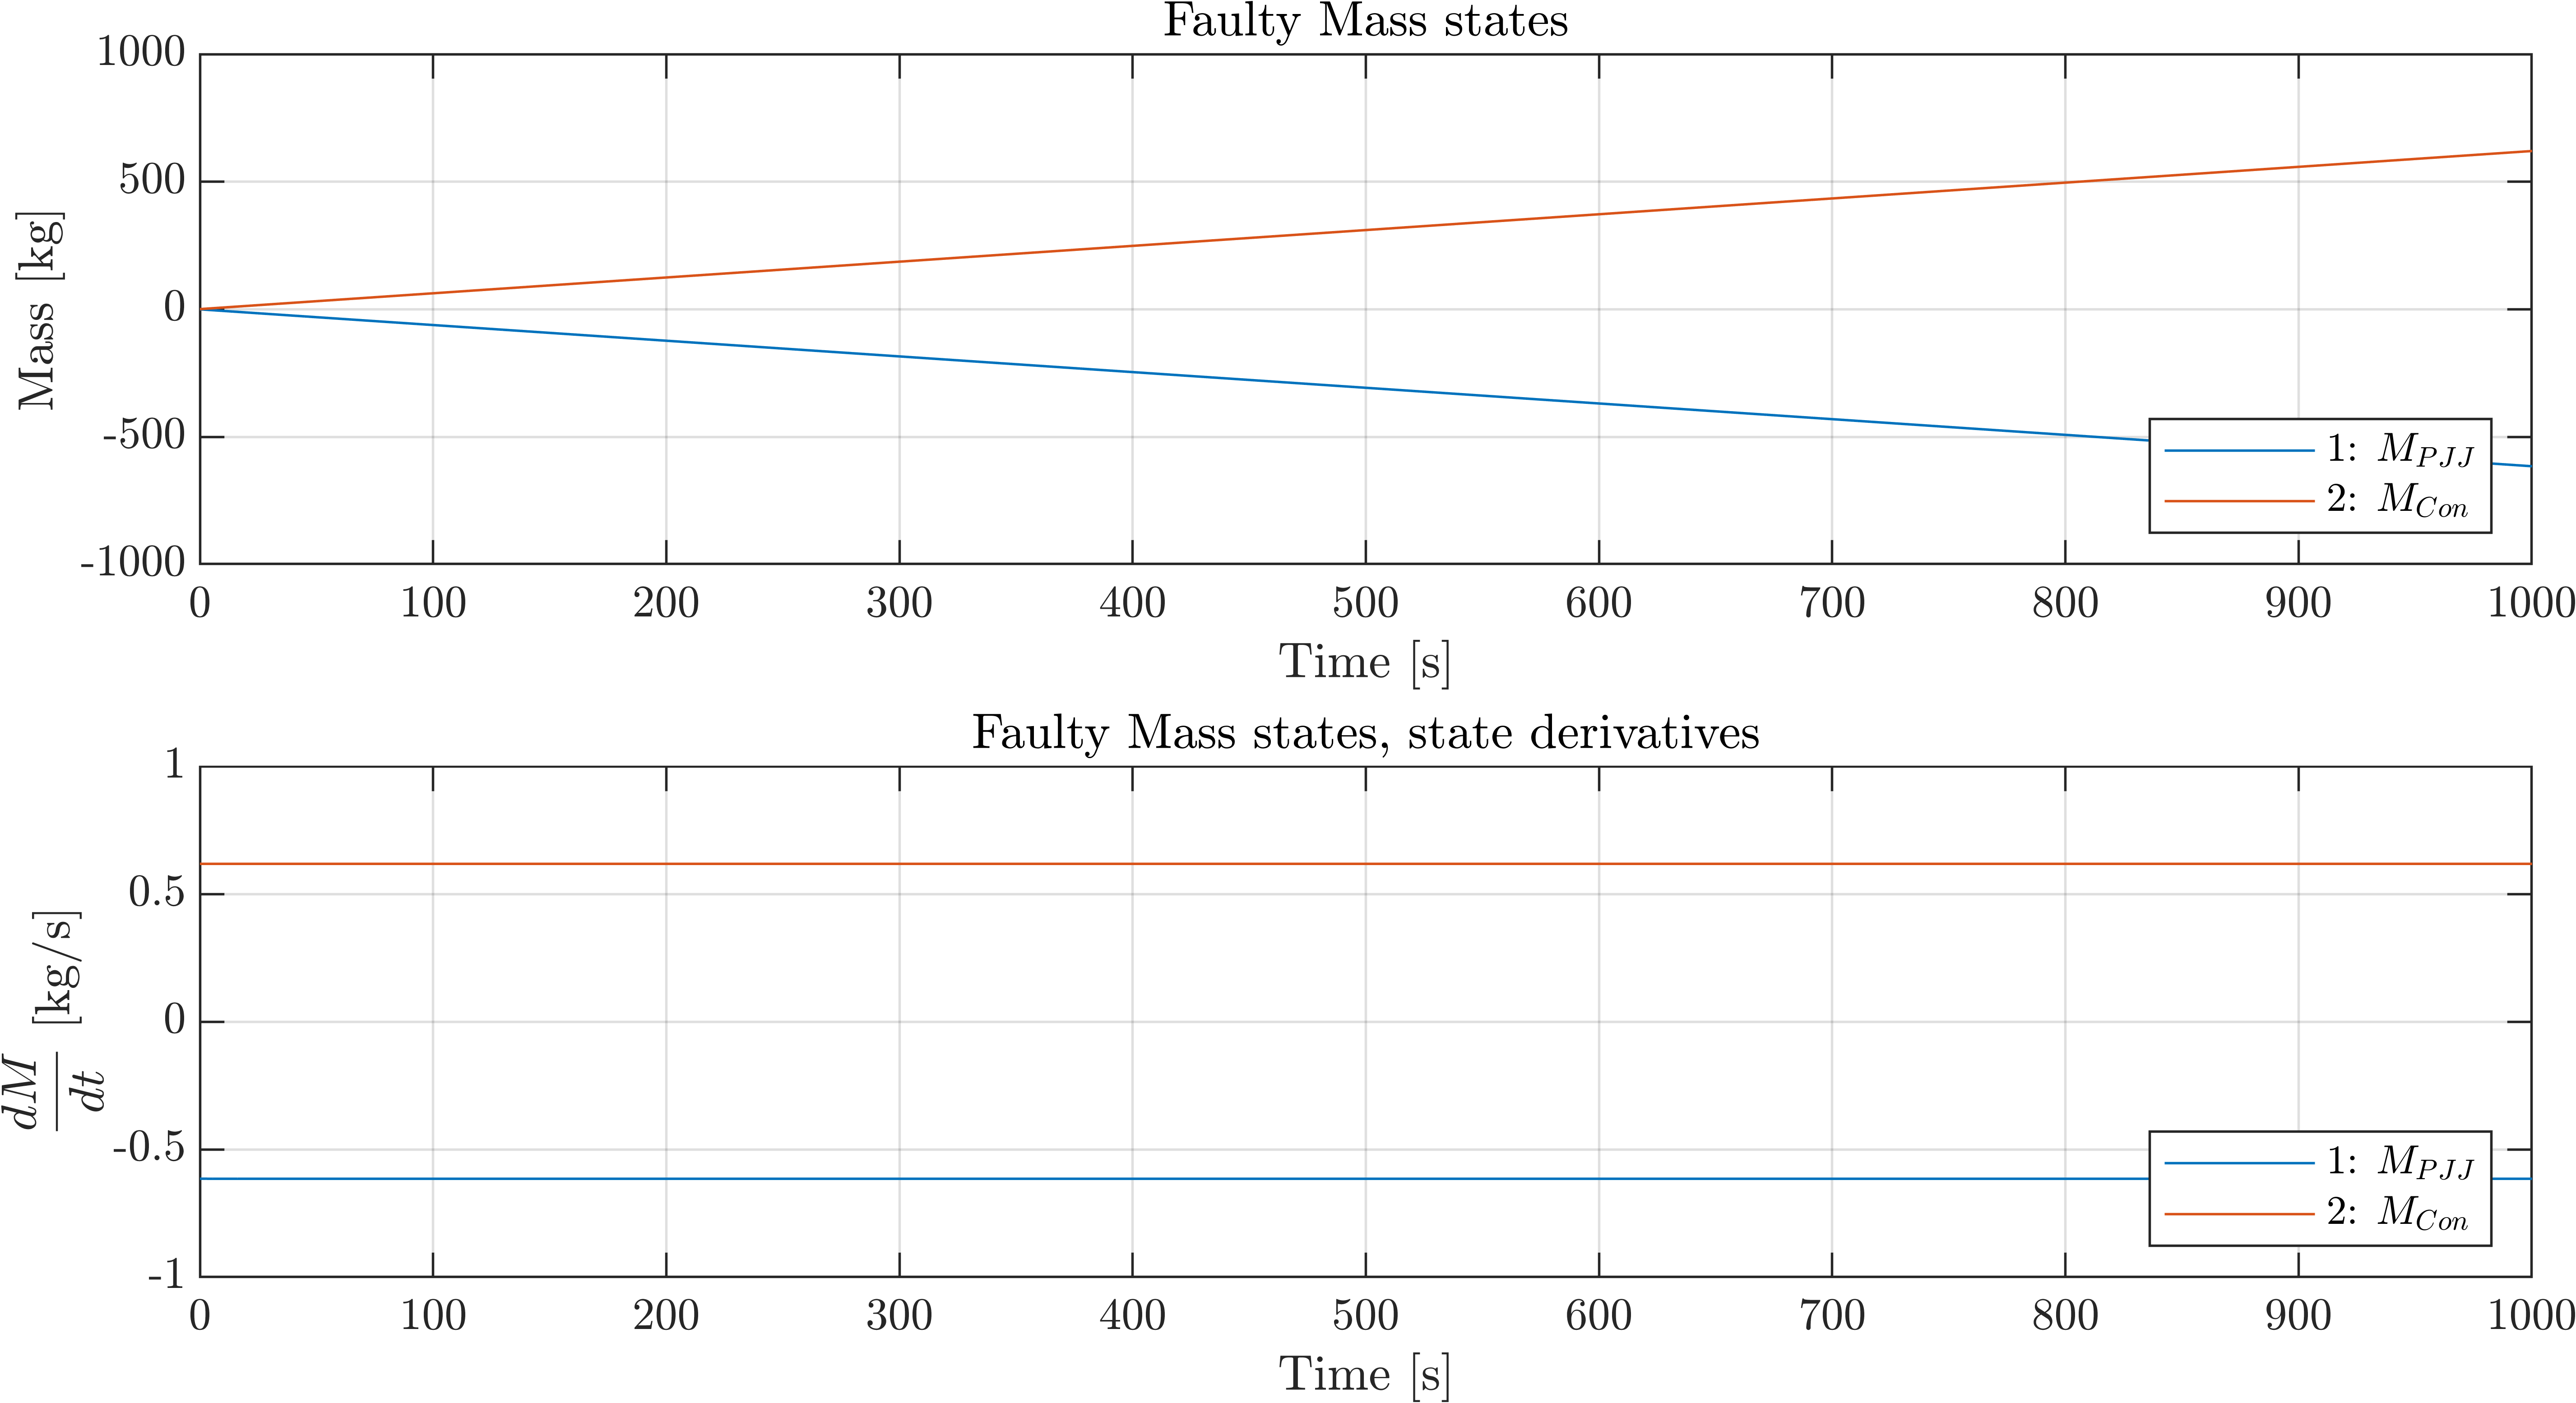
\includegraphics[width=1\textwidth]{Graphics/nonlin_sim_faulty_Mass.png}
	\caption{Plot of faulty states}
	\label{fig:non_lin_sim_faulty_Mass}
\end{figure}
This is due to some mismatches and simplifications in the modeling section. The issue is that the pressures inside the components are not defined as states, and such the masses does not affect the pressure and thereby the flows in the system. However, as a direct result of the missing link between the masses and the pressure, the masses in the Pipe Joining Junction and condenser are not affecting the rest of the system either. This can be verified by inspection in \cref{eq:f_noSub}, where it is seen that none of the states depend on $M_{pjj}$ and $M_{con}$. Resultingly the faulty states can excluded from the model as they do no affect any of the other states. Therefore the model as whole is not disregarded at this time. Even if the model poorly represents the physical system it may still be a candidate for a control model when linearised. \\

The next states to be investigated are the refrigerant masses in respectively the liquid-vapor and the vapor control volume of the evaporator, $ M_{lv} $ and $ M_v $. Additionally, the air mass flow was included in the plot. The plot can be seen in \cref{fig:non_lin_sim_Mass_Mvfucked}. It is noted that the plot has two distinct y-axes to allow for the inclusion of the air mass flow as well.
\begin{figure}[h]
	\centering
	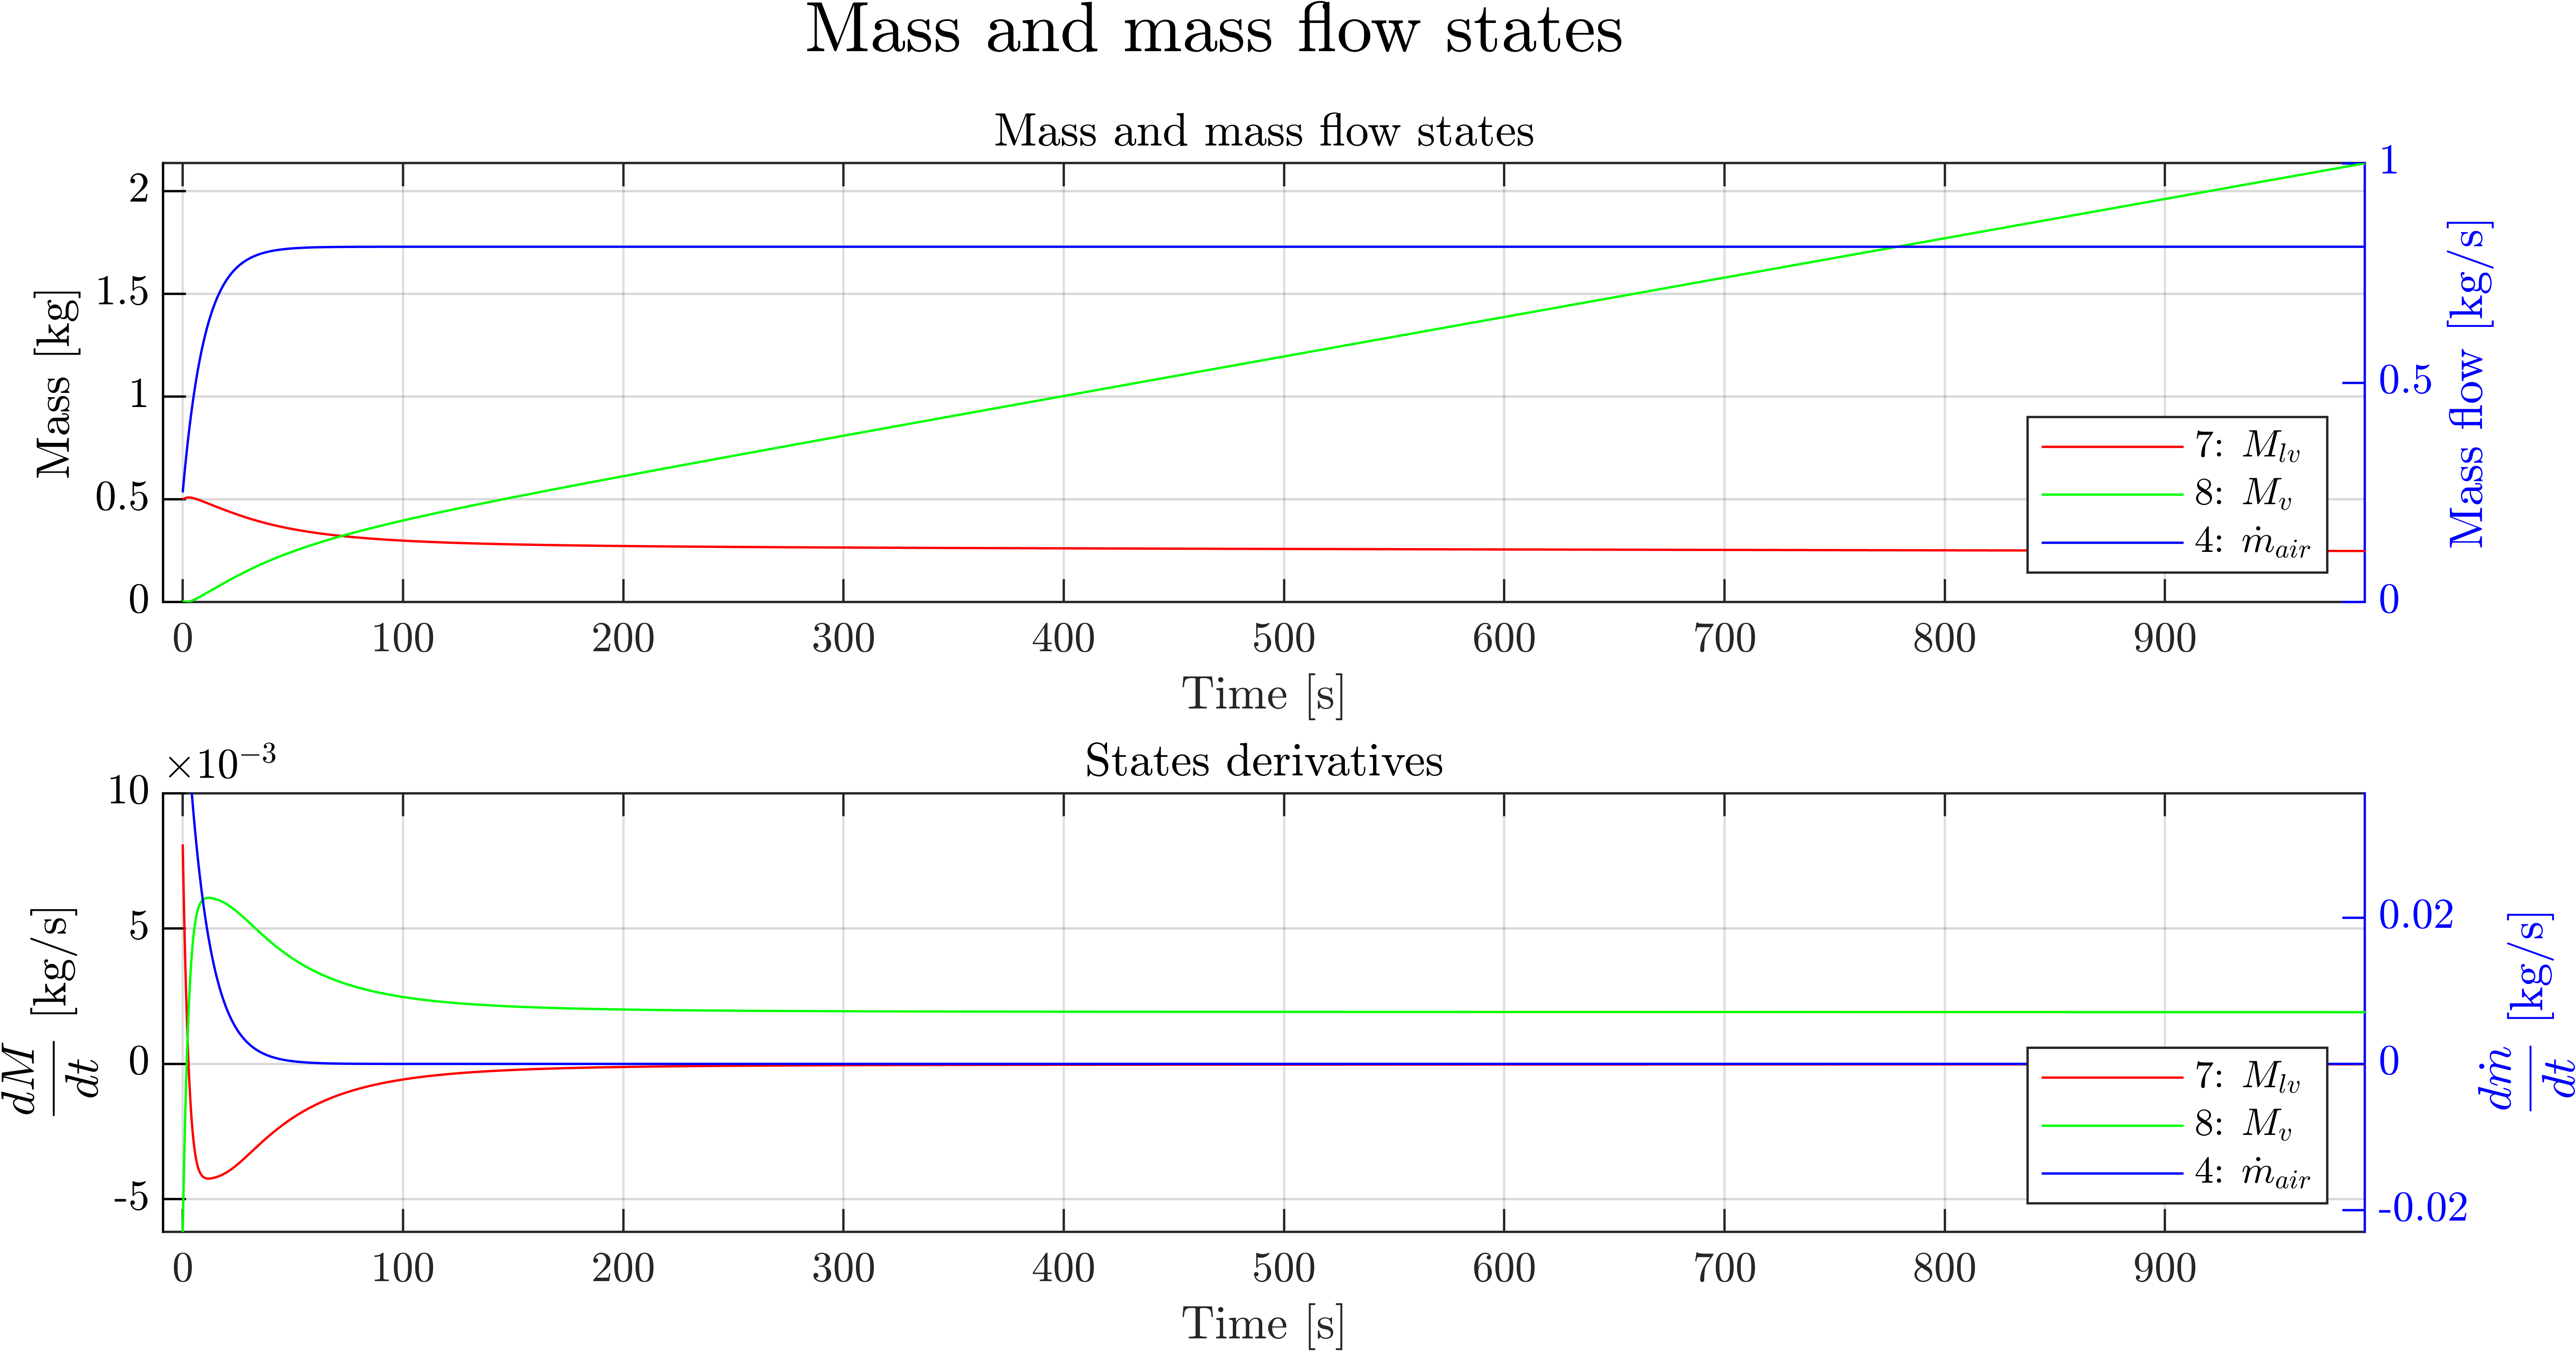
\includegraphics[width=1\textwidth]{Graphics/nonlin_sim_Mass_Mvfucked.png}
	\caption{Plot of states and state derivatives. Note the two y-axes. $ M_v $ appear to be integrating in subplot 1, with subplot two confirming that the state derivative is non-zero. Other states $ M_{lv} $ and $ \dot{m}_{air} $ converge to constant values in subplot 1.}
	\label{fig:non_lin_sim_Mass_Mvfucked}
\end{figure}
Observing the behavior of the state $ M_v $ reveals that  derivative of the state $M_v$ converges to a non-zero constant at around $ 3\cdot 10^{-3} $. This error makes the state integrate towards infinity. The error is considered as a numeric error as it does not make sense for the vapor mass to accumulate indefinitely. Therefore the phenomenon was investigated and measures were taken to handle the numerical error.

The non-zero offset of the derivative of $ M_v $ was discovered to be a function of the compressor speed. This function is simply subtracted from the derivative of the state $M_v$. This removed the integrating effect as can be seen in \cref{fig:non_lin_sim_Mass}, but may imply that some numerical errors were present in the non-linear model.
\begin{figure}[h]
	\centering
	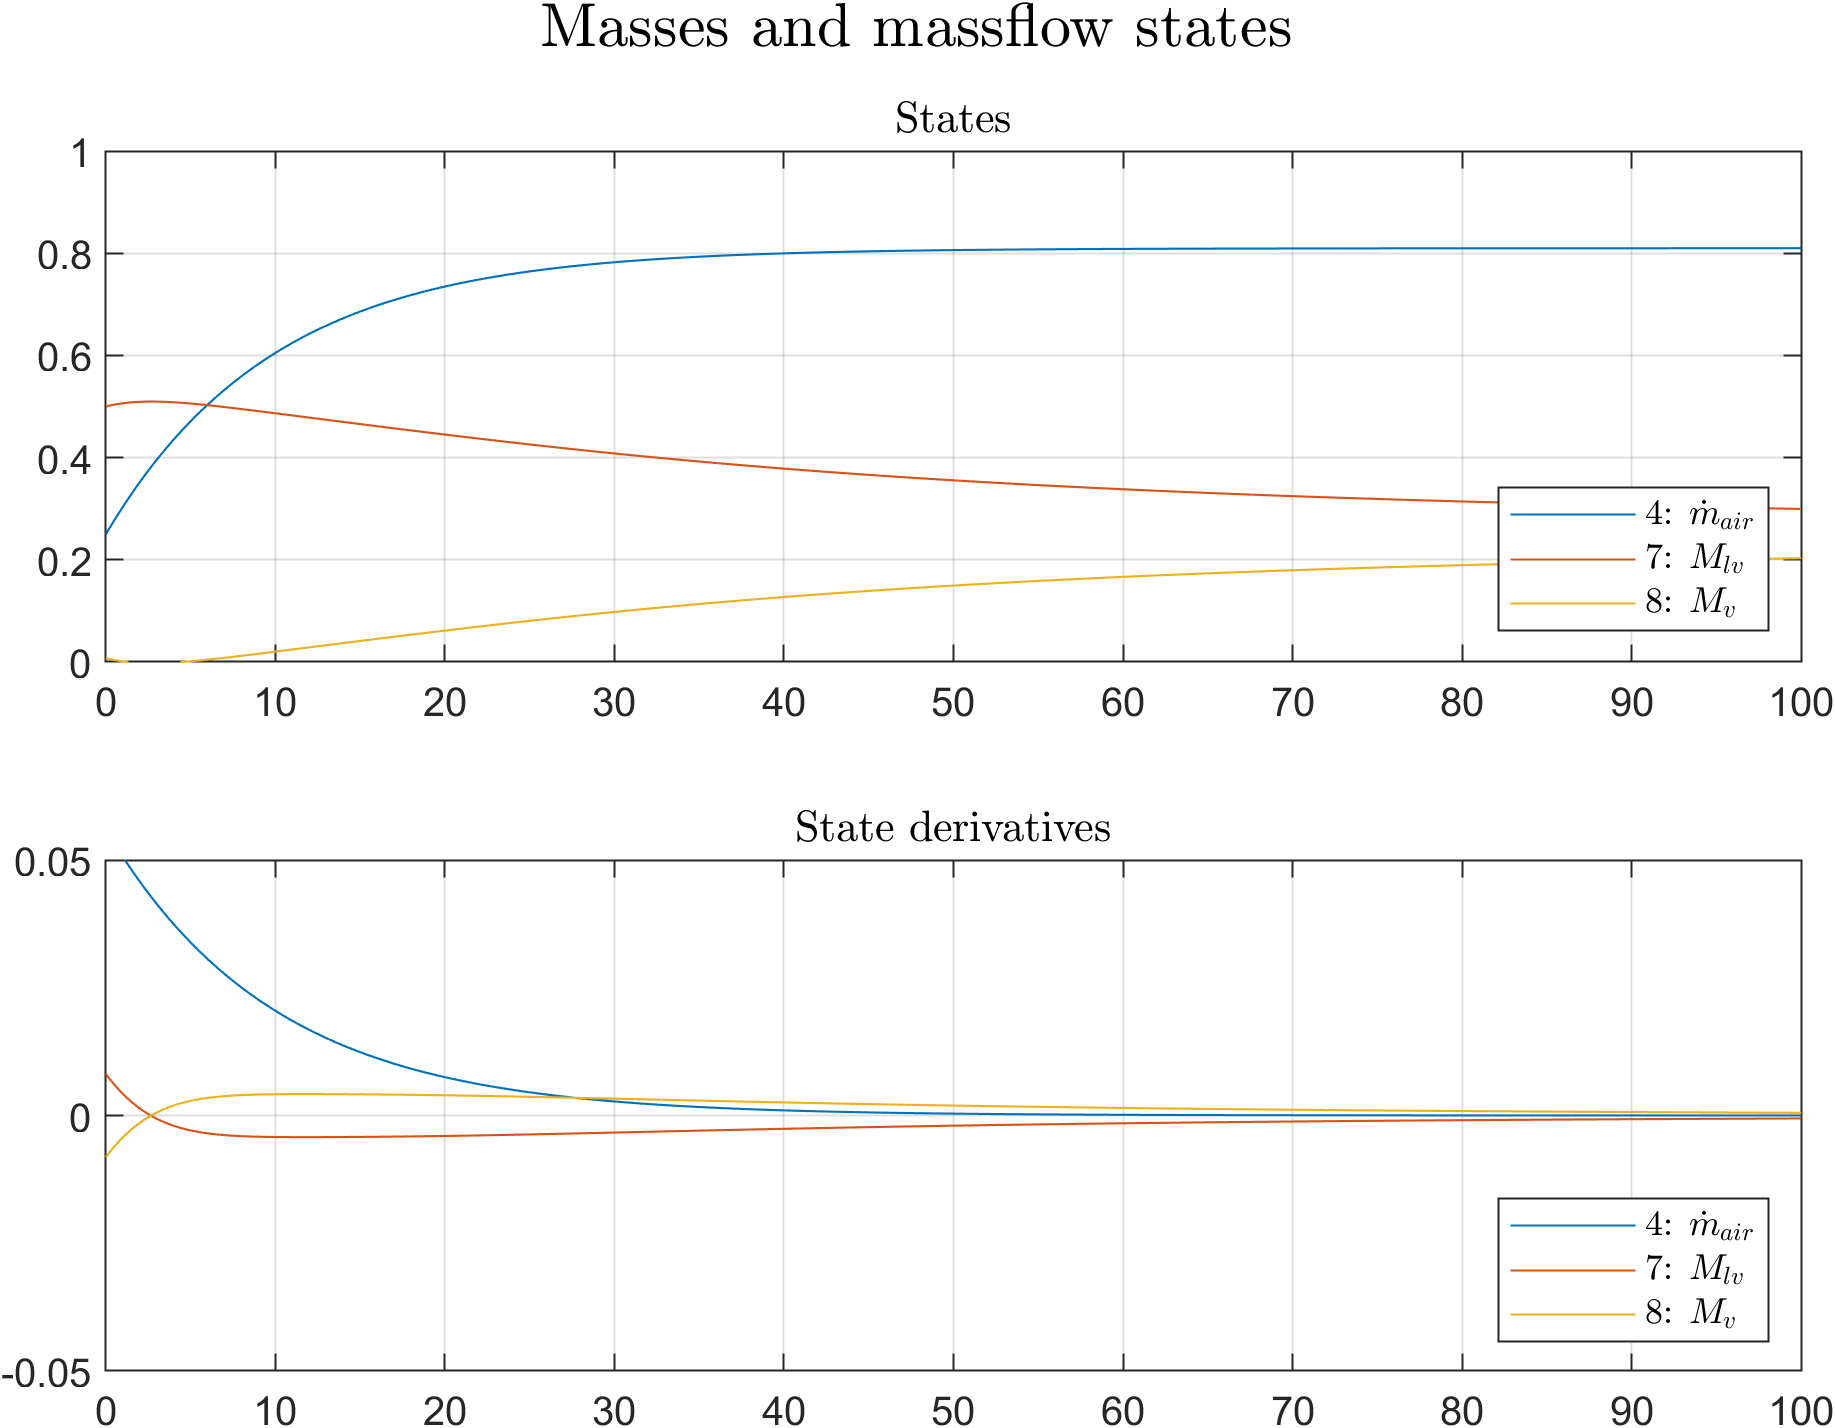
\includegraphics[width=1\textwidth]{Graphics/nonlin_sim_Mass.png}
	\caption{Plot of states $ M_v $, $ M_{lv} $ and $ \dot{m}_{air} $. Derivative of $ M_v $ is subtracted with a function of compressor speed $ \omega $. All states converge to constant values. Note the two y-axes.}
	\label{fig:non_lin_sim_Mass}
\end{figure}
\newpage
Further investegations of the phenomenon were performed but did not reveal the origin of the error. No further actions were thus taken.\\
After correcting the numerical error, all of the states in \cref{fig:non_lin_sim_Mass_Mvfucked} converges to a constant value and is thus considered to be stable.\\


Lastly in \cref{fig:non_lin_sim_Temperature}, all of the temperature states are plotted. They all converge to a constant value, indicating stable behavior.
\begin{figure}[h]
	\centering
	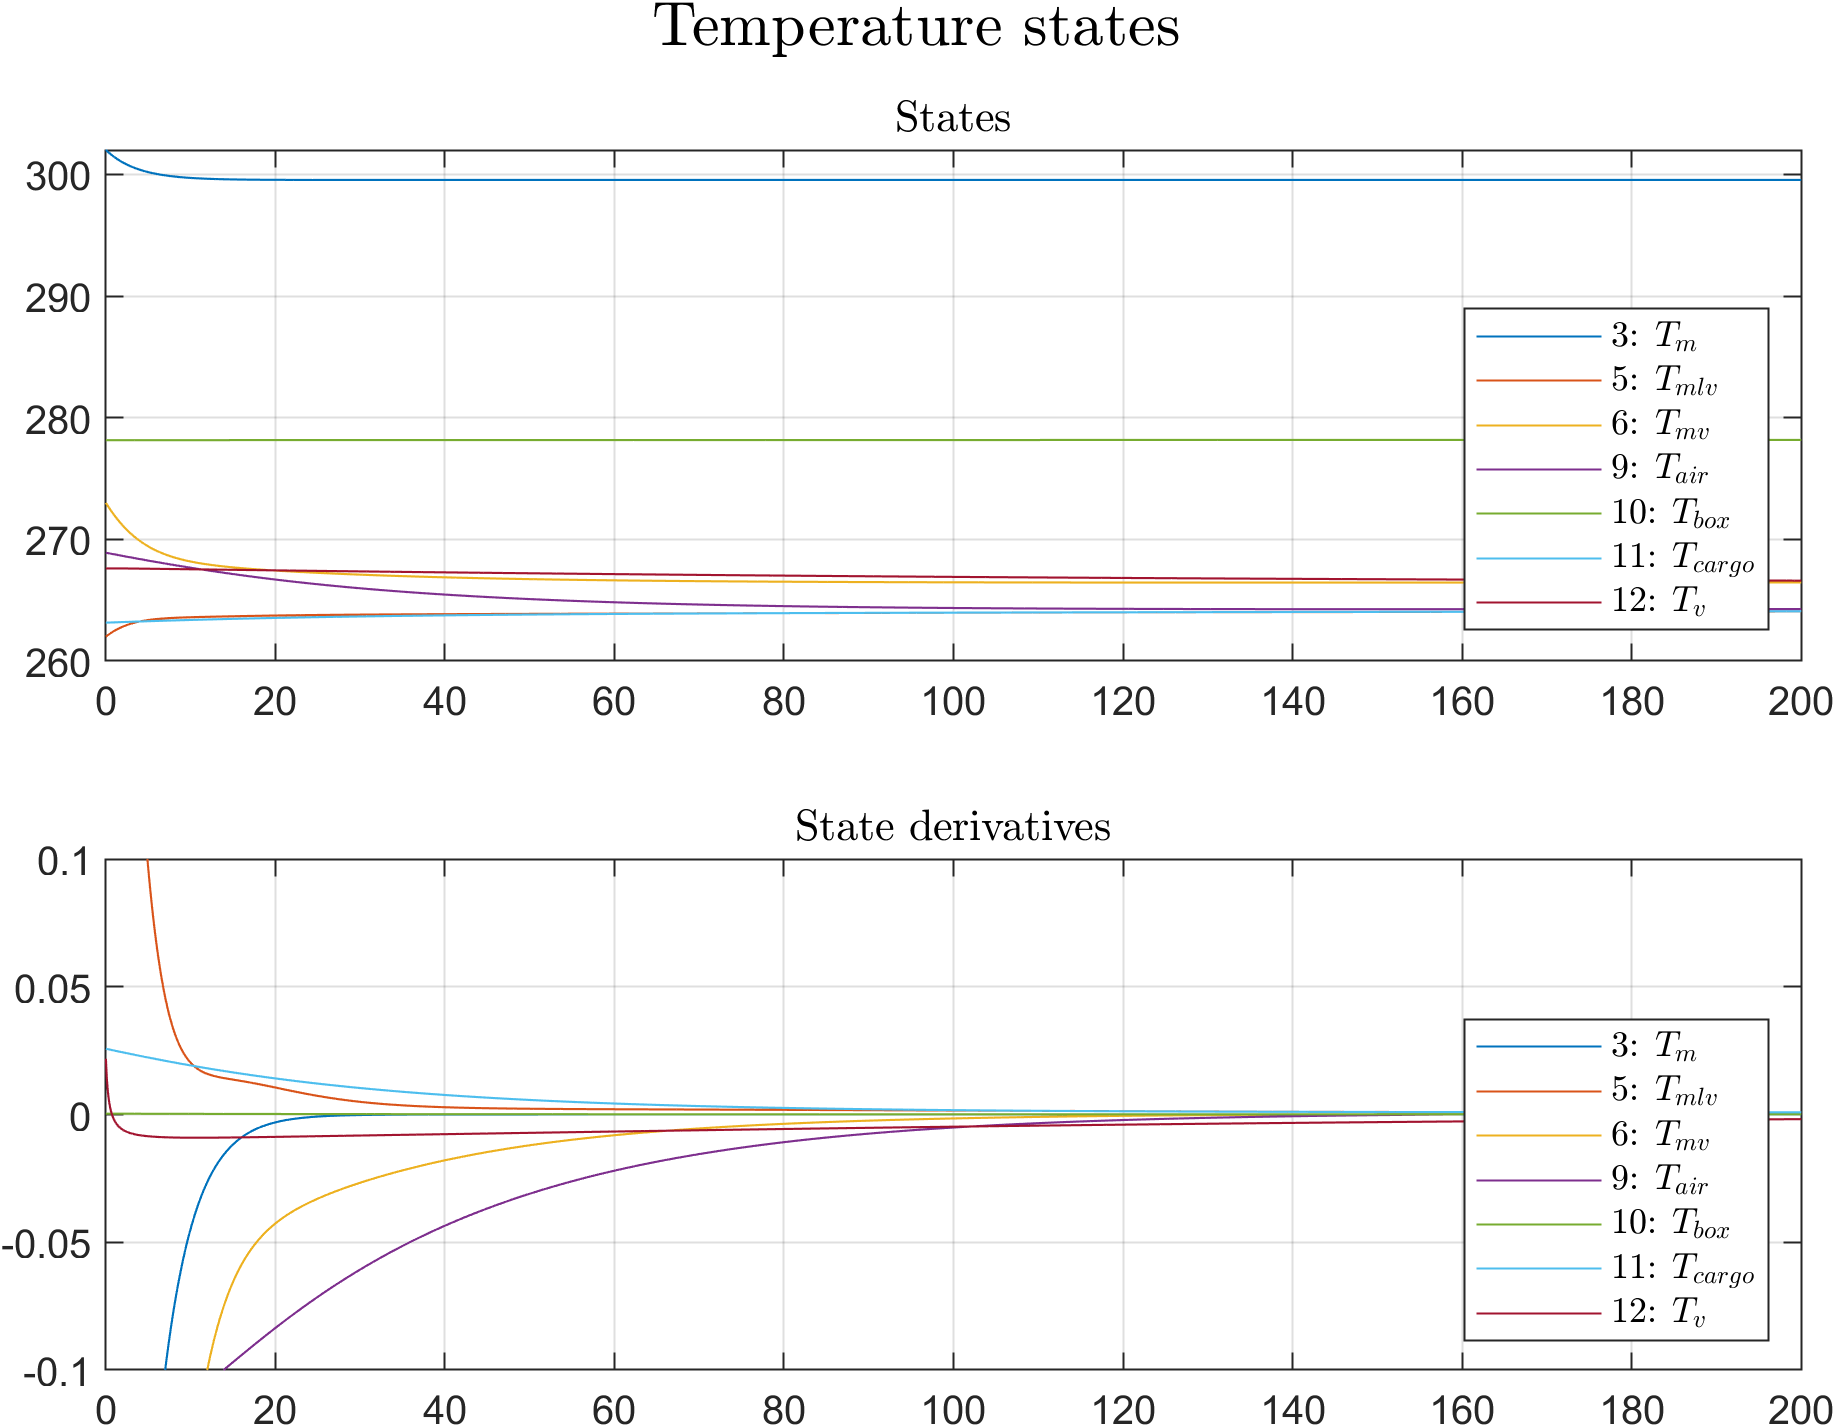
\includegraphics[width=1\textwidth]{Graphics/nonlin_sim_Temperature.png}
	\caption{Plot of all the temperature states. The states are collected into 3 subplots, where the first coverge faster than the second, and the second faster than the third. All the temperature states converge to a constant value}
	\label{fig:non_lin_sim_Temperature}
\end{figure}
\newpage
Now that all of the states has been investigated, a preliminary conclusion on whether the non-linear state space model in \cref{eq:f_noSub} can be verified to be stable remains to be drawn. Based on the states in \cref{fig:non_lin_sim_faulty_Mass} it could be concluded that the model is not stable and accurate enough. However, as mentioned earlier, the two involved states are not affecting the rest of the model. Furthermore, as the states $ M_{pjj} $ and $ M_{con} $ are not output and thereby wished to be controlled, it is decided to just omit these two states from our model.
This leaves the model with 2 fewer states, which can be considered favorable since the states does not provide extra information on the controlled outputs. The rest of the states converge to constant values, indicating stability for the model. This allows for the next step in the process, which is linearisation.

Note: in \cref{app:tj_2}, an alternative modeling approach was investigated, to mitigate the errors in \cref{fig:non_lin_sim_faulty_Mass}.


%The control inputs are:

%\begin{center}
%	\begin{tabular}{l p{10cm}}
%		$ \Theta_1 $  & The valve opening degree of the \\
%		$ \Theta_2 $  & The valve opening degree of the \\
%		$ U_{fan_1} $ & The condenser fan speed         \\
%		$ U_{fan_2} $ & The evaporator fan speed        \\
%		$ \omega $    & The compressor speed
%	\end{tabular}
%\end{center}

%The disturbance is:

%\begin{center}
%	\begin{tabular}{l p{10cm}}
%		$ T_{ambi} $  & The ambient air temperature
%	\end{tabular}
%\end{center}